\documentclass[ngerman]{article}

\usepackage[utf8]{inputenc}
\usepackage{default}
\usepackage[ngerman]{babel}
\usepackage{amsmath,amsfonts,amssymb}
\usepackage{graphicx}
\usepackage{multicol}
\usepackage{txfonts}



\title{Mikroskopische Modelle stochastischer Dynamik}
\date{}
\author{Michael Meyer}
\begin{document}

 \maketitle


\setlength\parindent{0pt}

\begin{section}{Brownsche Bewegung}


Ein makroskopisches Teilchen der Masse $m$ und Geschwindigkeit $v$ bewege sich in einer Flüssigkeit.
  
Die Stöße mit den Molekülen der Flüssigkeit bewirken eine mittlere bremsende Kraft auf das Teilchen und eine fluktuierende stochastische Kraft $f(t)$. 

Die Bewegungsgleichung lautet dann
(Langevinsche Gleichung):
   $$m\frac{\text{d}^{2}\mathbf{x}}{\text{d}t^{2}}=-\alpha \frac{\text{d}\mathbf{x}}{\text{d}t}  + f(t)$$
 

Die Brownsche Bewegung kann man  durch den \textit{ random walk} beschreiben.



 1-dimensionaler random walk:
\begin{itemize}
\item
Teilchen bewegt sich nach links oder rechts mit gleicher Wahrscheinlichkeit
\item
Jede Einzelbewegung ist unabhängig von den Bewegungen zuvor
\end{itemize}

Sei die Distanz einer Bewegung $a$, $r$ die Anzahl der Bewegungen nach rechts und $n$ die Gesamtanzahl der Bewegungen.
Dann befindet sich das Teilchen am Ort
$$x = a(r-(n-r))= a(2r-n) \Rightarrow r= \frac{n}{2}+\frac{x}{2a}$$

Ist die Dauer einer elementaren Bewegung $\tau$, dann ist die Zeit für $t$ für $n$ Sprünge $$t=n \tau$$

Die Wahrscheinlichkeit bei $n$ Einzelbewegungen $r$-mal nach rechts zu gehen ist 
$$ P(r, n)=\binom{n}{r} \left(  \frac{1}{2}\right)^r \left(  \frac{1}{2}\right)^{n-r}=\binom{n}{r}\left(  \frac{1}{2}\right)^n  = \binom{t / \tau}{t/ (2\tau) + x/(2a)} \left(  \frac{1}{2}\right)^{t/\tau}$$




Ersetzt man den Binominialkoeffizienten durch Fakultäten und verwendet die Stirlingsche Formel ( $n!=e^{-n}n^n\sqrt{2\pi n}$ ) erhält man näherungsweise
$$P(a, \tau, t)=2(2\pi t)^{-1/2}\tau^{1/2}e^{-x^2\tau/(2a^2t)}$$

Uns interessiert jedoch $\int_{x1}^{x2}P(x, t)\text{d}x$. 


Dafür benutzen wir $\sum_{r1}^{r2}P(r, t)\approx \int_{r1}^{r2}P(r, t)\text{d}r$ und d$r=\frac{1}{2a}\text{d}x$
$$ \int_{x1}^{x2}\frac{\tau^{1/2}}{a}(2\pi t)^{-1/2}e^{-x^2\tau/(2a^2t)}\text{d}x$$
Wir definieren $\frac{\tau^{1/2}}{a}\coloneqq D^{-1/2}  \stackrel{!}{=} const$ und erhalten $$\int_{x1}^{x2} (2\pi Dt)^{-1/2}e^{-x^2/(2Dt)}\text{d}x$$

\begin{figure}[h]
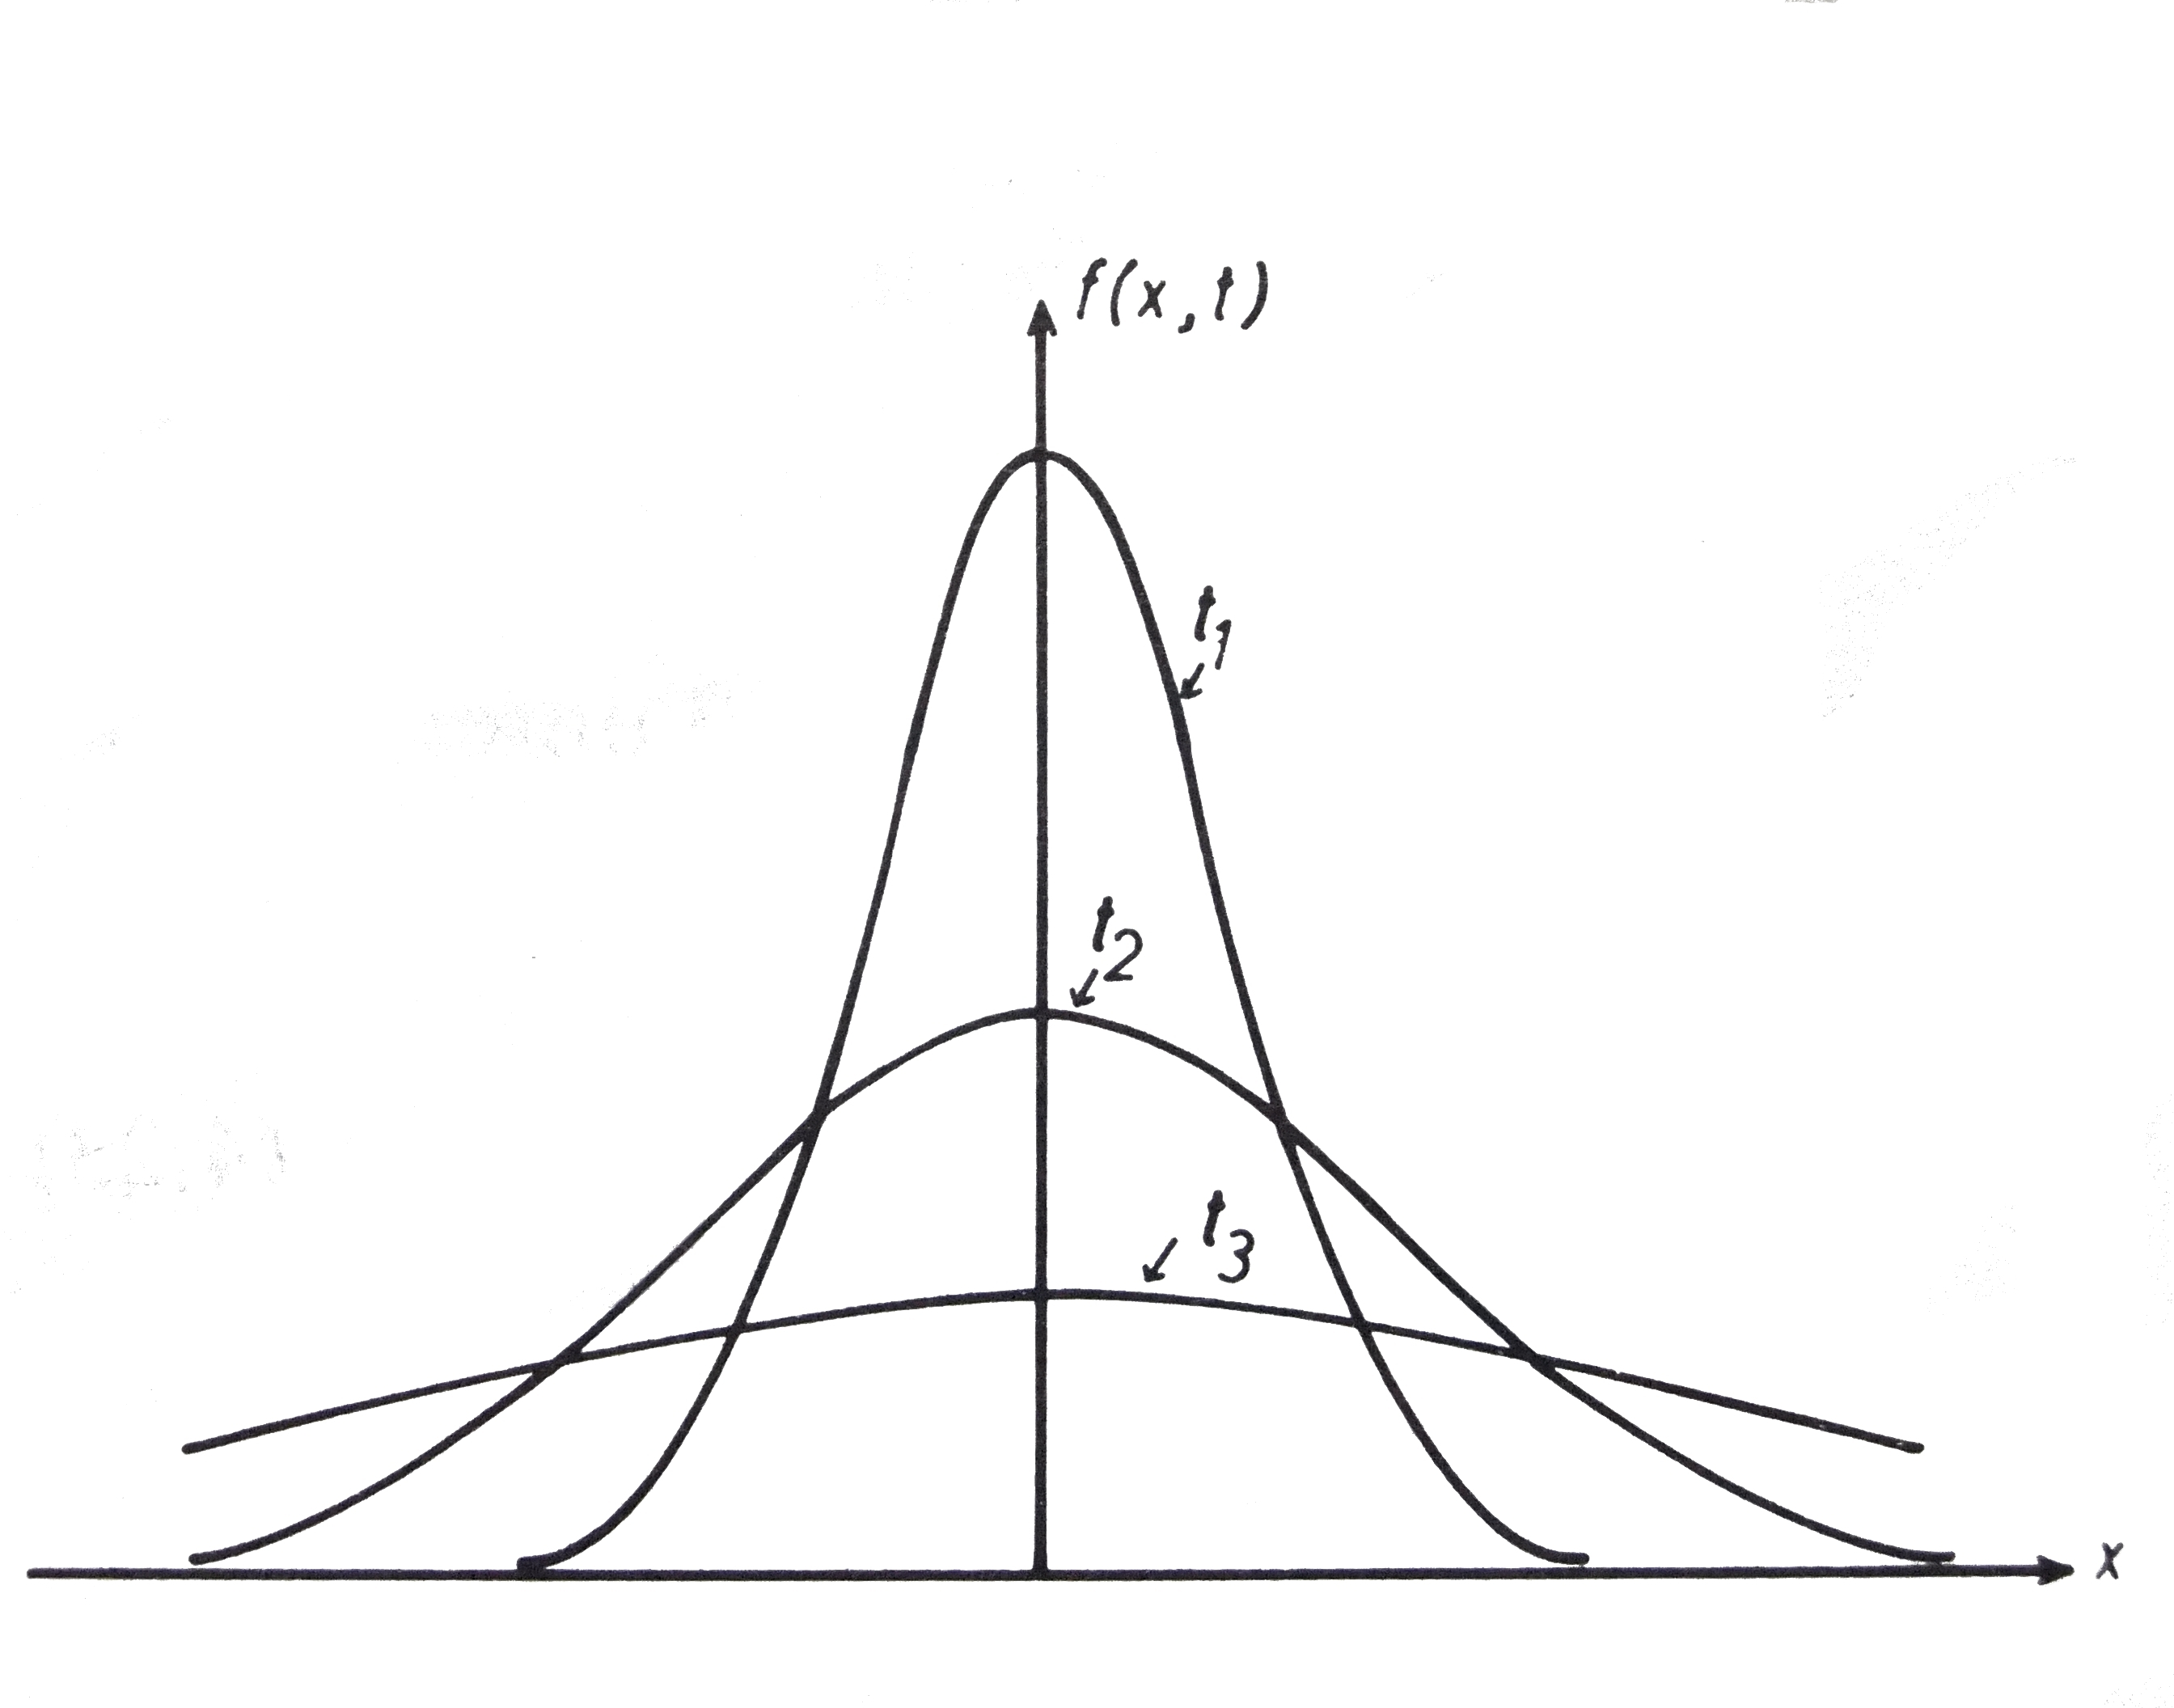
\includegraphics[width=4.5cm]{verteilung.JPG}
\caption{Die Funktion $f(x,t)= (2\pi Dt)^{-1/2}e^{-x^2/(2Dt)}$ zu drei verschiedenen Zeiten als Funktion der Ortskoordinate $x$}
\end{figure}



Offensichtlich gilt $<x>=0$. 

Um $<x^2>$ zu berechnen, gehen wir zurück zur Langevin-Gleichung
$$m\frac{\text{d}^{2}{x}}{\text{d}t^{2}}=-\alpha \frac{\text{d}{x}}{\text{d}t}  + f(t)$$ und multiplizieren beide Seiten mit x:
$$mx\frac{\text{d}{\dot x}}{\text{d}t}=m\left[\frac{\text{d}}{\text{d}t}(x\dot x)-\dot x^2\right]=-\alpha x \frac{\text{d}{x}}{\text{d}t}  + x f(t)$$





Wir nehmen auf beiden Seiten den Mittelwert
$$m\left< \frac{\text{d}}{\text{d}t}(x\dot x)\right>=m\frac{\text d}{\text d t}<x\dot x>=k_{\mathrm{B}}T-\alpha <x\dot x>$$ und erhalten eine einfache Differentialgleichung mit der Lösung: $$<x\dot x> = Ce^{-\gamma t}+\frac{k_{\mathrm B}T}{\alpha}     \text{    \            \                   mit } \gamma :=\frac{\alpha}{m}$$Durch die Anfangsbedingung: Teilchen zur Zeit $t=0$ bei $x=0$ lässt sich die Integrationskonstante bestimmen. $ 0=C+\frac{k_{\mathrm B}T}{\alpha} \Rightarrow C=\frac{-k_{\mathrm B}T}{\alpha}$ Setzt man C in die Gleichung ein, erhält man:
$$<x\dot x> =\frac{1}{2} \frac{\text d}{\text d t}<x^2>= \frac{k_{\mathrm B}T}{\alpha} (1-e^{-\gamma t})$$ Nochmalige Integration ergibt 
$$<x^2>=\frac{2k_{\mathrm B}T}{\alpha}[t-\gamma^{-1}(1-e^{-\gamma t})]$$





\end{section}

\begin{section}{Boltzmann-Gleichung}

 


 Die Verteilungsfunktion $ f(\boldsymbol{x}, \boldsymbol{v}, t)$  ist definiert durch
 $$  f( \boldsymbol{x}, \boldsymbol{v}, t)  \text{d}^3x \  \text{d}^3v =  \begin{cases} \text{Anzahl der Teilchen im Phasenraum-} \\ \text{volumen d $^3x$ d $^3v$  bei $\boldsymbol{x}, \boldsymbol{v}$ zur Zeit $t$. } \end{cases} $$
 Also gilt:
		$$ \int \text{d}^3x \  \text{d}^3v \ f(\boldsymbol{x}, \boldsymbol{v}, t) = N $$


\begin{figure}[h]
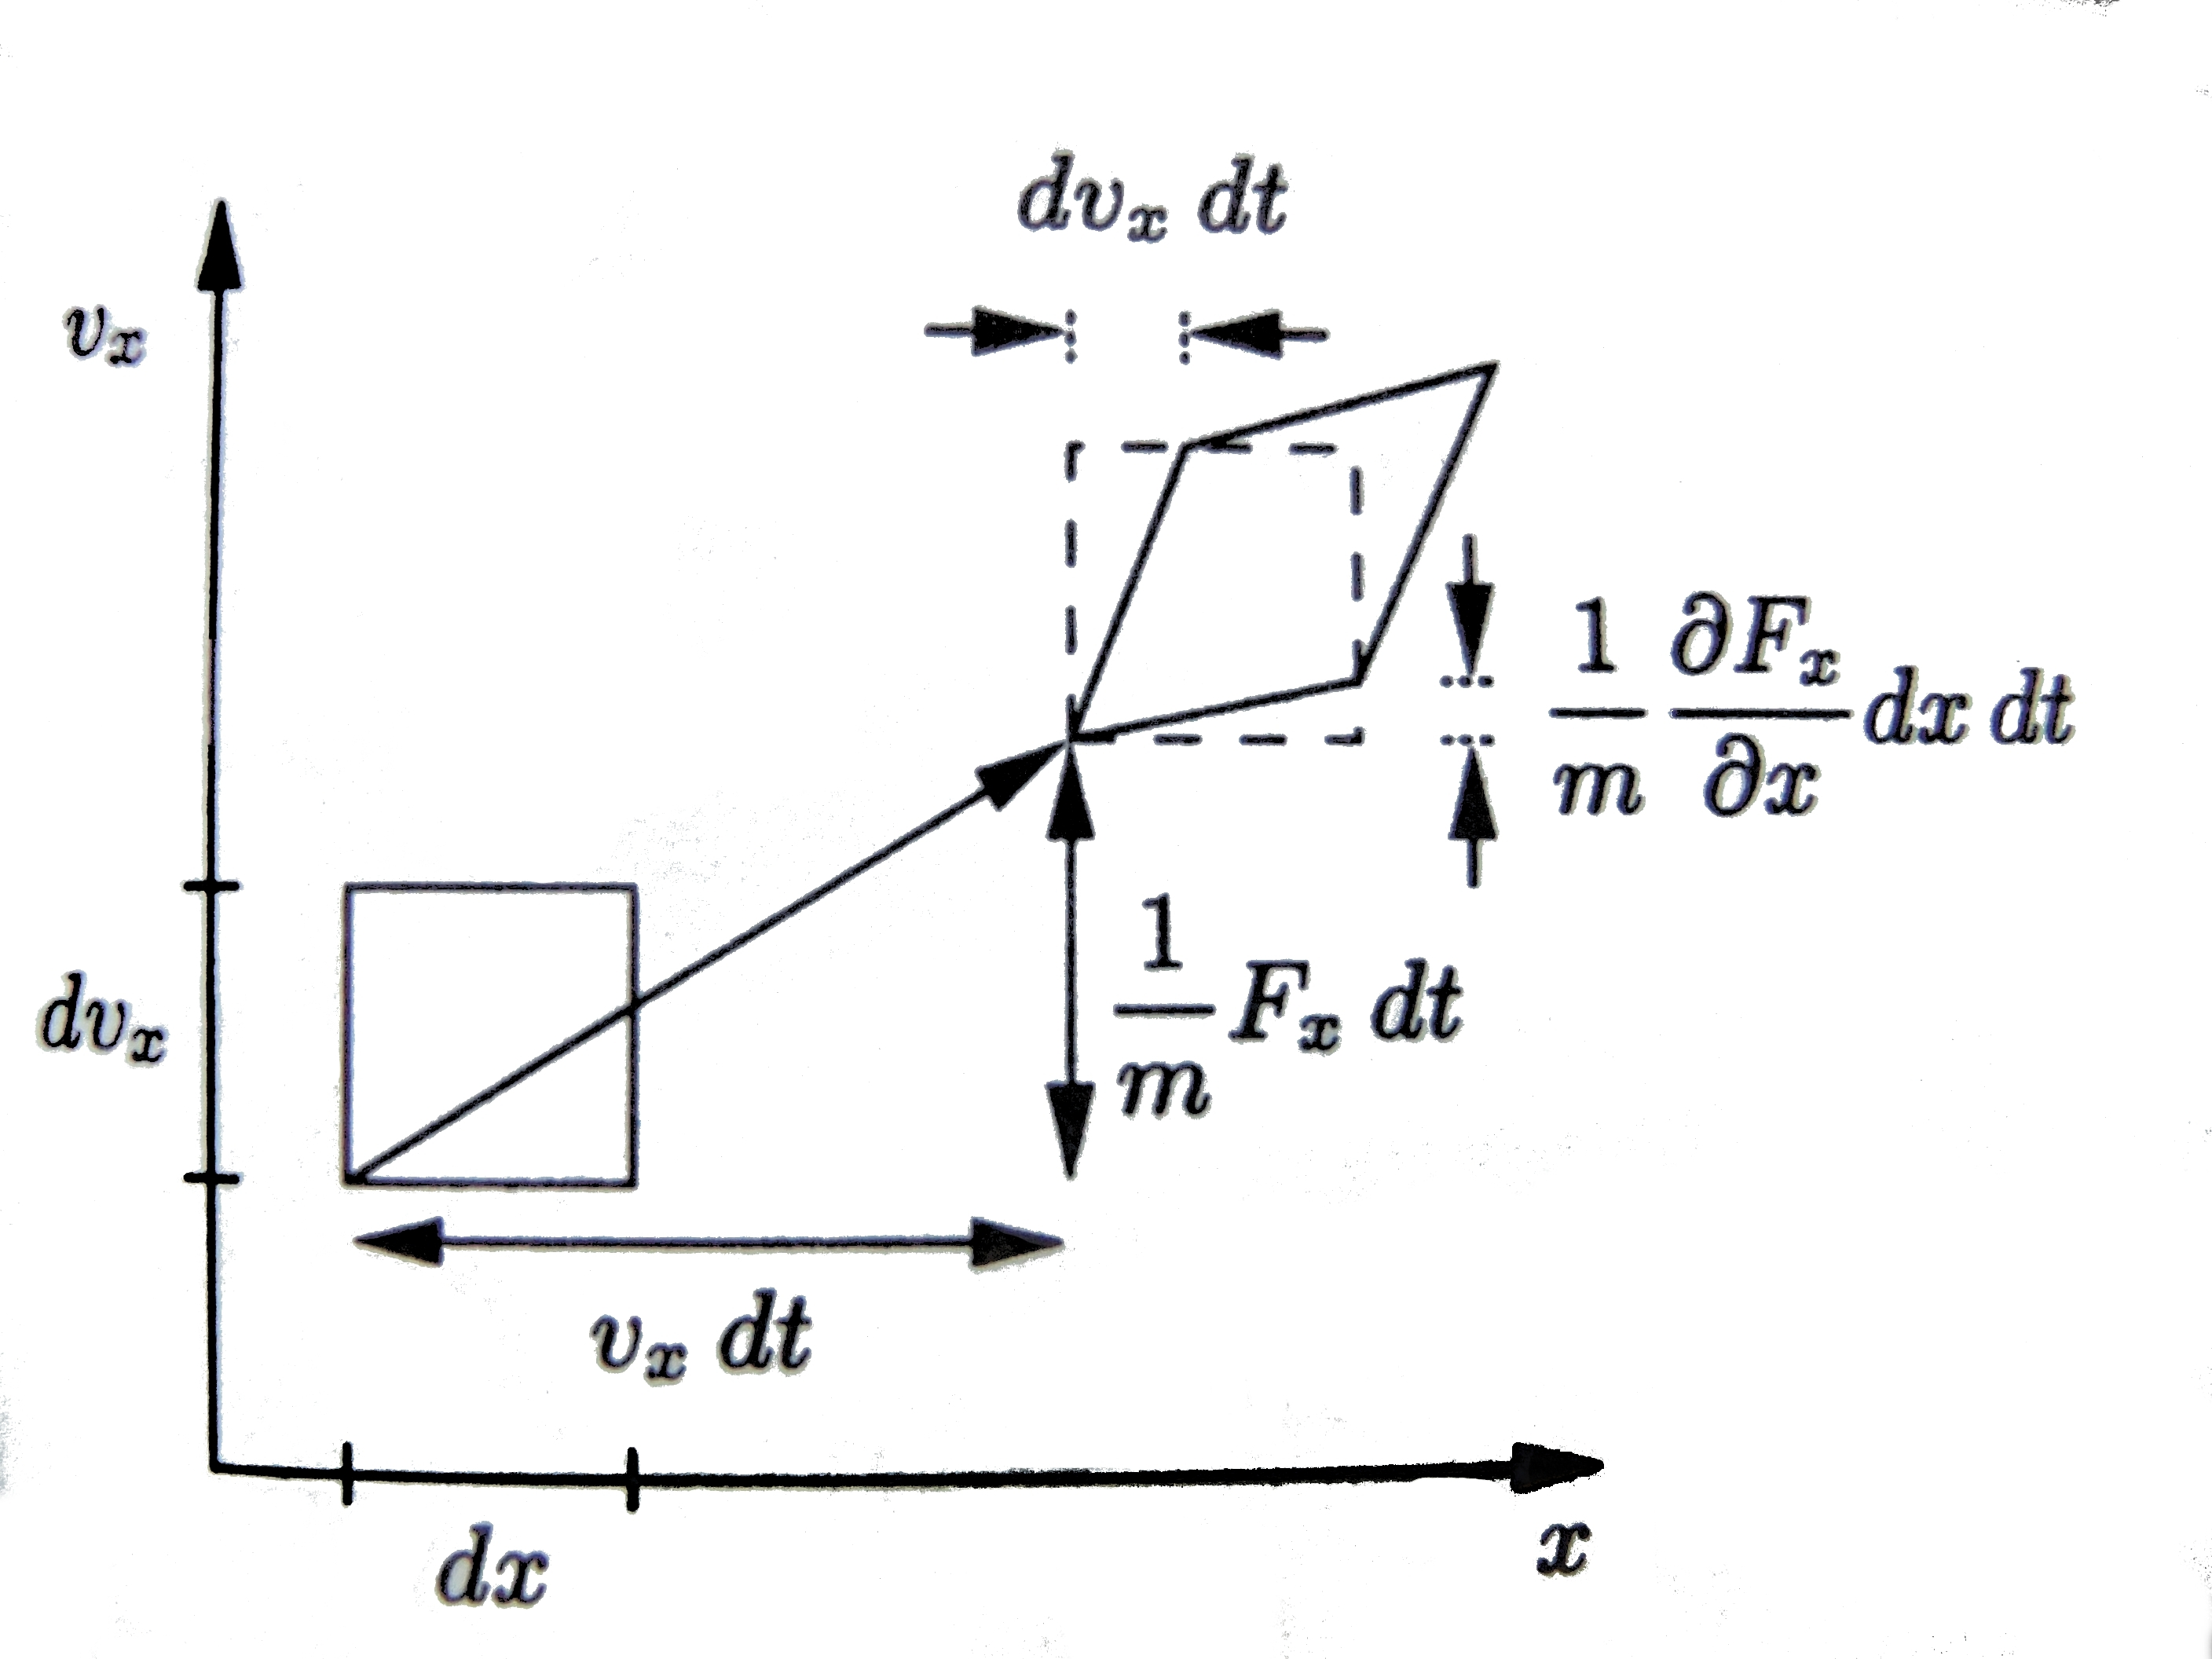
\includegraphics[width=5.5cm]{boltzmann.JPG}
\caption{
Deformation eines Volumenelements im $ \mu$-Raum während des Zeitintervalls d$t$}
\end{figure}
Jedoch gilt: d$^3x'\text{d}^3v'= \text{d}^3x\text{d}^3v$ 






Die Zahl der Teilchen zur Zeit $t$ in d$^3x$d$^3v$  ist $$ f( \boldsymbol{x}, \boldsymbol{v}, t)  \text{d}^3x \text{d}^3v$$
und die Zahl der Teilchen in dem daraus nach dem Zeitintervall d$t$ entstehenden Volumenelement ist $$f\left(\boldsymbol{x}+\boldsymbol{v} \text{d}t, \boldsymbol{v} + \frac{\boldsymbol{F}}{m} \text{d}t, t + \text{d}t\right) \text{d}^3x' \text{d}^3v'$$




Die Differenz  kann nur durch Stöße entstehen: $$\left[f\left(\boldsymbol{x}+\boldsymbol{v} \text{d}t, \boldsymbol{v} + \frac{\boldsymbol{F}}{m} \text{d}t, t + \text{d}t\right) - f\left( \boldsymbol{x}, \boldsymbol{v}, t\right) \right] \text{d}^3x \text{d}^3v = \left.\frac{\partial f}{\partial t}\right|_\mathrm{Stoss} \text{d}t\text{d}^3x \text{d}^3v$$



Die Entwicklung dieser Bilanz ergibt:
    
        
     
     $$   \underbrace{\left( \boldsymbol{v} \cdot \frac{\partial}{\partial \boldsymbol{x}} + \frac{\boldsymbol{F}}{m} \cdot \frac{\partial}{\partial \boldsymbol{v}}+\frac{\partial}{\partial t}\right)}_{\frac{\text{d}}{\text{d}t}} f(\boldsymbol{x}, \boldsymbol{v}, t) =  \left.\frac{\partial f}{\partial t}\right|_\mathrm{Stoss}
    $$



Sei $W(\boldsymbol{v},\boldsymbol{v}_2;\boldsymbol{v}_3,\boldsymbol{v}_4)$ die Übergangswahrscheinlichkeit $ \boldsymbol{v},\boldsymbol{v}_2  \rightarrow \boldsymbol{v}_3,\boldsymbol{v}_4$


Aufgrund der Zeiumkehrinvarianz der Streuung gilt: $W(\boldsymbol{v},\boldsymbol{v}_2;\boldsymbol{v}_3,\boldsymbol{v}_4)= W(\boldsymbol{v}_3,\boldsymbol{v}_4; \boldsymbol{v},\boldsymbol{v}_2)$


Die Zahl der Stöße (vereinfacht: nur 2-Teichen-Stöße), die aus dem betrachteten Volumenelement herausführen ist proprtional zu:
\begin{itemize}


\item
der Zahl der Teilchen mit Geschwindigkeit $\boldsymbol{v}$

\item
der  Zahl der Teilchen mit Geschwindigkeit $\boldsymbol{v}_2$
\item
$W(\boldsymbol{v},\boldsymbol{v}_2;\boldsymbol{v}_3,\boldsymbol{v}_4)$
\end{itemize}
Analog ist die Zahl der Stöße, die in das Volumenelement hereinführen proportional zu der Anzahl der Teilchen mit Geschwindigkeit $\boldsymbol{v}_3$, zur Zahl der Teilchen mit Geschwindigkeit $\boldsymbol{v}_4$ und $W(\boldsymbol{v},\boldsymbol{v}_2;\boldsymbol{v}_3,\boldsymbol{v}_4)$.



Daraus ergibt sich:
$$ \left.\frac{\partial f}{\partial t}\right|_\mathrm{Stoss} =  \int \text{d}^3v_2 \ \text{d}^3v_3 \ \text{d}^3 v_4 W(\boldsymbol{v},\boldsymbol{v}_2;\boldsymbol{v}_3,\boldsymbol{v}_4) \cdot \left[ f(\boldsymbol{x},\boldsymbol{v}_3,t)f(\boldsymbol{x},\boldsymbol{v}_4,t) - f(  \boldsymbol{x}, \boldsymbol{v},t)f(\boldsymbol{x},\boldsymbol{v}_2,t) \right]  $$



Boltzmann-Gleichung 
	$$ \left( \boldsymbol{v} \cdot \frac{\partial}{\partial \boldsymbol{x}} + \frac{\boldsymbol{F}}{m} \cdot \frac{\partial}{\partial \boldsymbol{v}}+\frac{\partial}{\partial t}\right) f(\boldsymbol{r}, \boldsymbol{v}, t) =  \left.\frac{\partial f}{\partial t}\right|_\mathrm{Stoss}     $$ $$ \left.\frac{\partial f}{\partial t}\right|_\mathrm{Stoss} =  \int W(\boldsymbol{v},\boldsymbol{v}_2;\boldsymbol{v}_3,\boldsymbol{v}_4) \cdot\left[ f(\boldsymbol{x},\boldsymbol{v}_3,t)f(\boldsymbol{x},\boldsymbol{v}_4,t) - f(  \boldsymbol{x}, \boldsymbol{v},t)f(\boldsymbol{x},\boldsymbol{v}_2,t) \right] \text{d}^3v_2 \ \text{d}^3v_3 \ \text{d}^3 v_4 $$

  


 
 
\end{section}


\begin{thebibliography}{4}
\bibitem{a} Fließbach, Torsten (2012):
Lehrbuch zur theoretischen Physik/4, 5. Aufl.

\bibitem{d}
Haken, Hermann (1990):
Synergetik, 3. Aufl.

\bibitem{c}
Reif, Frederick (1987):
Statistische Physik und Theorie der Wärme, 3. Aufl.

\bibitem{b} Schwabl, Franz (2006):
Statistische Mechanik, 3. Aufl.




\end{thebibliography}
 









\end{document}
